\chapter{Sammanfattning p{\aa} svenska}\noindent

Mankind has always had a fascination with looking at the infinitely
small. Since the invention of microscope people have been trying to find ways to
look at smaller and smaller things. Optical microscopy is incredibly useful but
its resolution is fundamentally limited by the wavelength of visible light, which
around 400nm for violet light. 

The invention of X-ray crystallography in
the beginning of the twentieth century made it possible to observe the
structures of things much smaller than the wavelength of visible light. X-ray
typically used in crystallography have a wavelength of 1 \AA, 4000 times smaller
than violet light. This means it is possible to observe things that are that
much smaller. 

Unfortunately X-rays have a few disadvantages compared to visible
light, the most important of all is that its refraction index is always very
close to 1 which means that in practise it is impossible to build conventional
lenses and so we cannot have an exact analogue to the optical
microscope. Instead of capturing an image of an object the best we can do is
capture its diffraction pattern. The diffraction pattern is very different from
the image of the object but under certain circunstances it is possible to
recover the image of the object from its diffraction pattern, a procedure known
as phasing. The difficulty in phasing is that it is not possible to determine
the object that gave rise to a certain diffraction pattern directly. Instead one
has to calculate the diffraction pattern from many objects until it finds one
that fits the experimental diffraction pattern. In effect we are replacing the
lens from the optical microscope by a computer (see Fig. \ref{Fig:lens_computer}).

\begin{figure}[ht]
\centering
  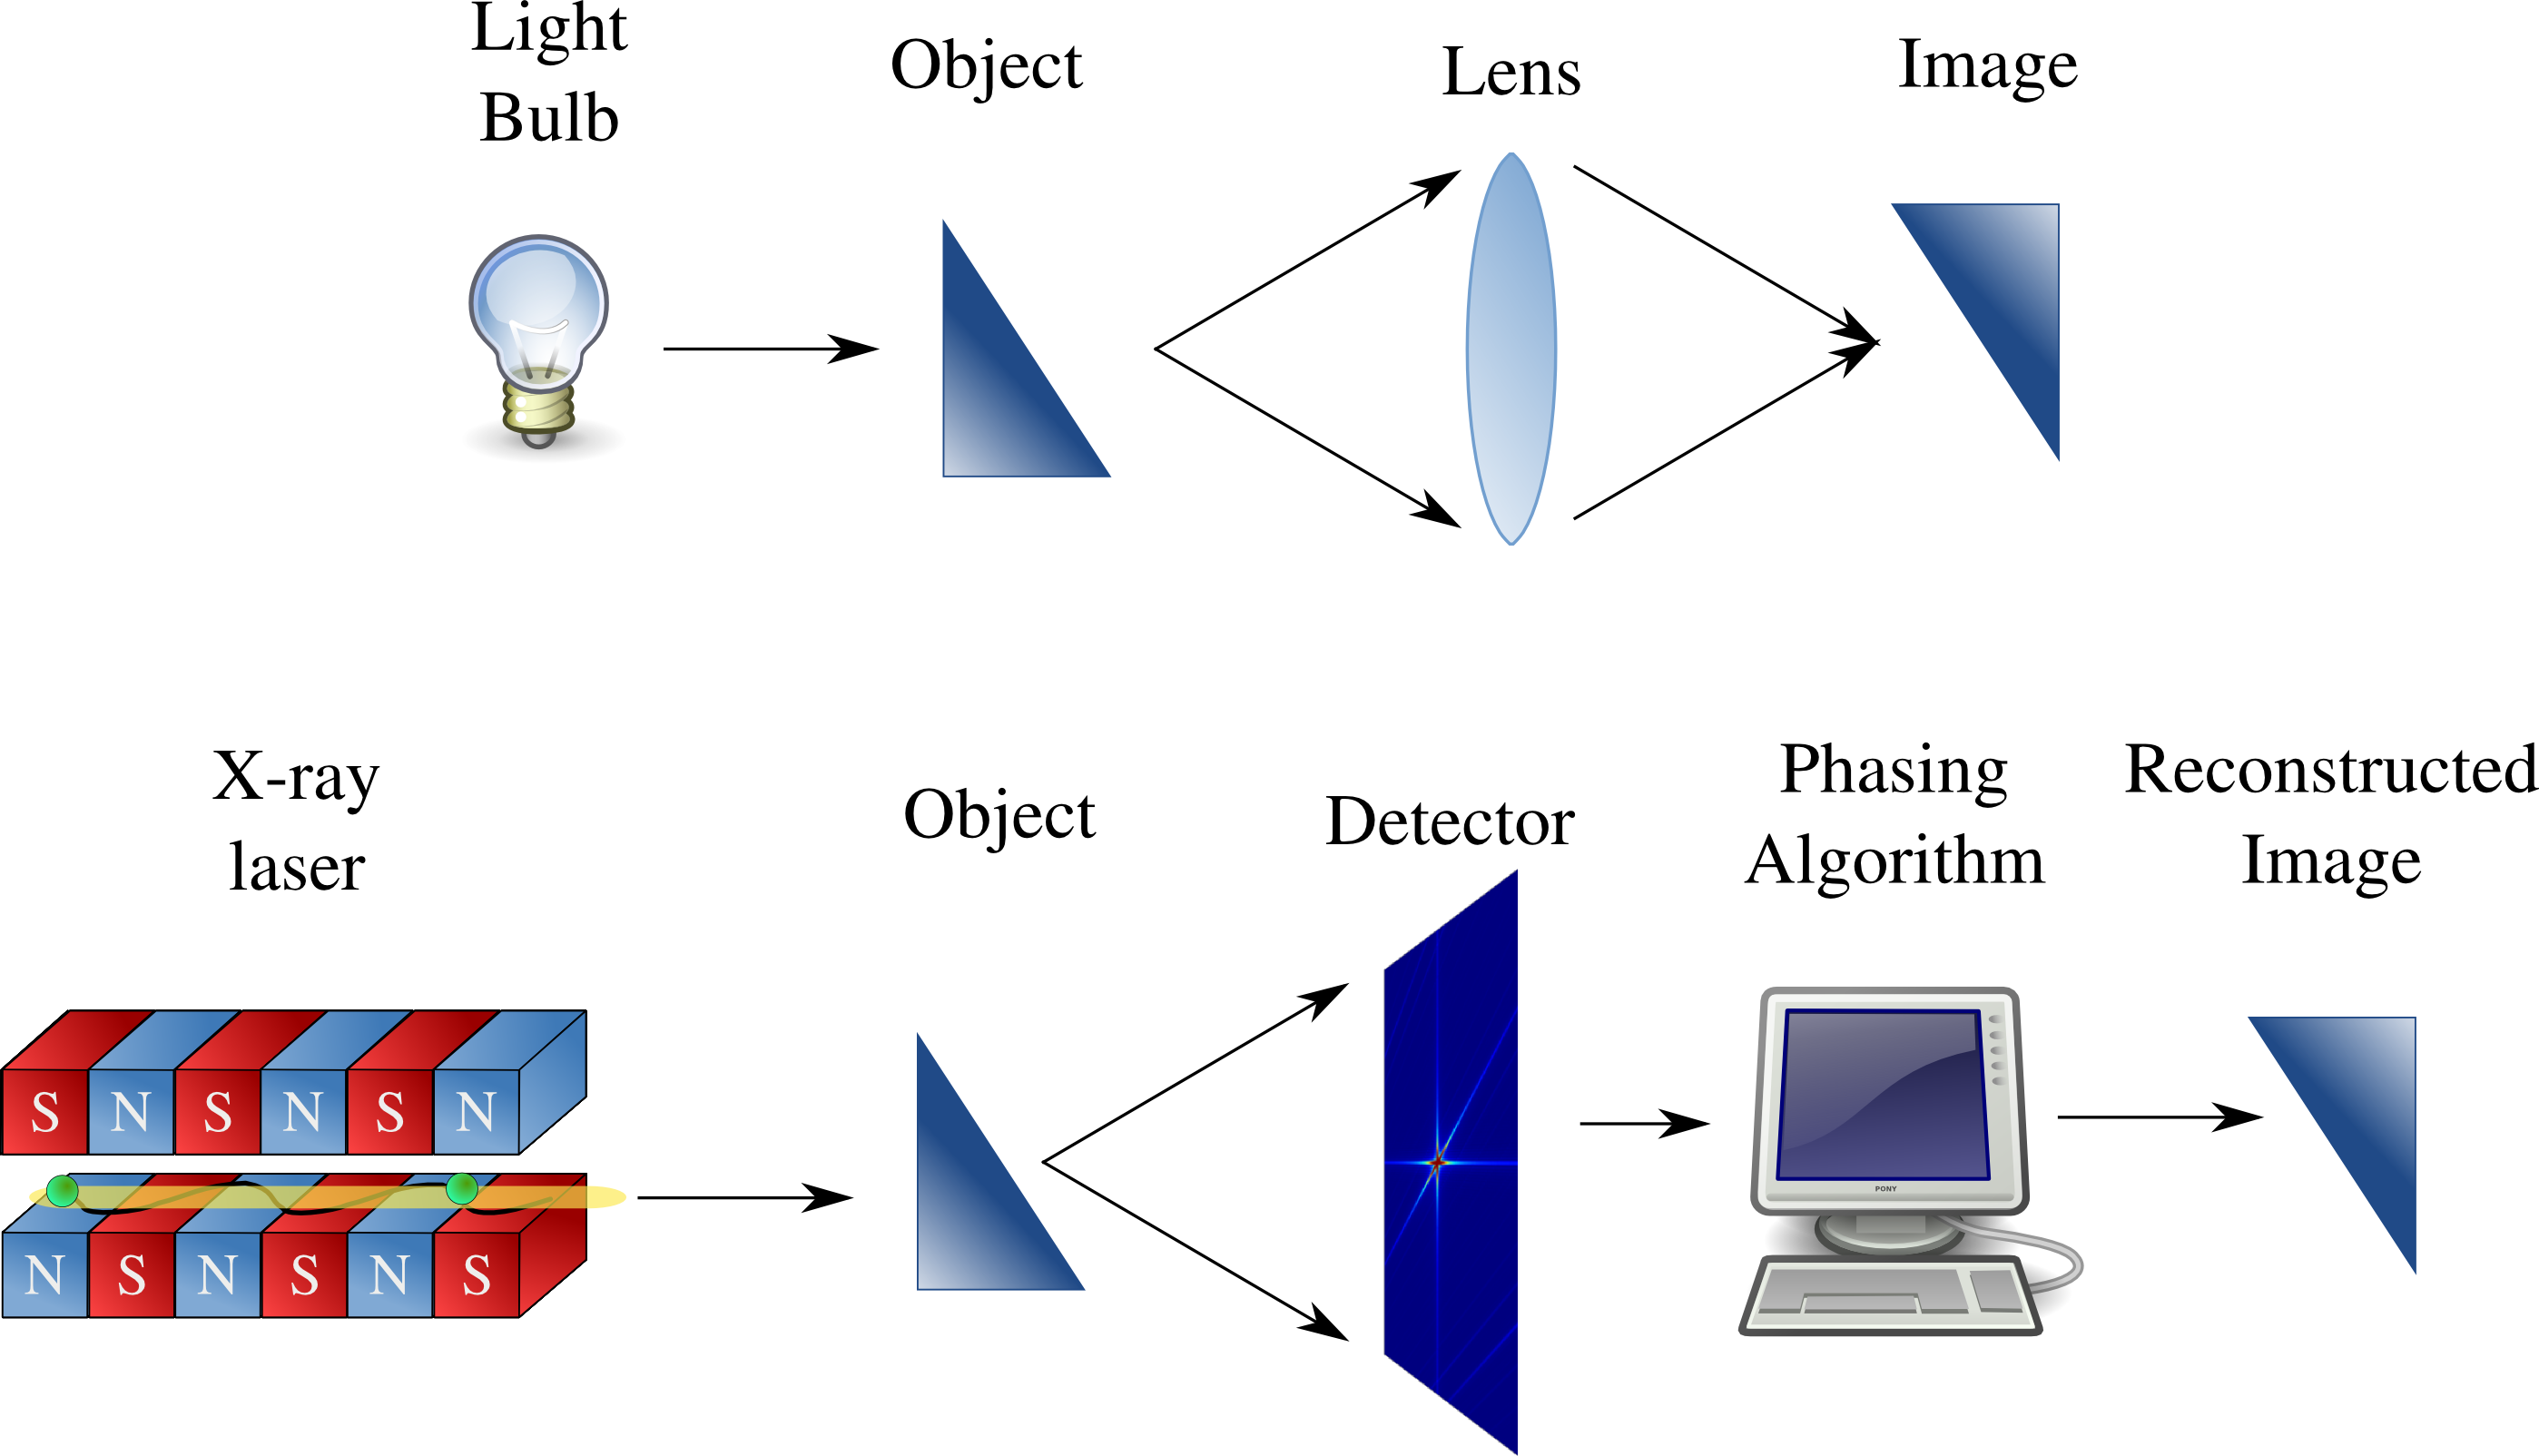
\includegraphics[width=1.0 \columnwidth]{lens_computer_analogy.png}
  \caption{Comparison of microscopy imaging using a lens and diffractive
    imaging, where the lens is replaced by a phasing algorithm executed by a computer. }
  \label{Fig:lens_computer}
\end{figure}

Another difficulty of imaging very small structures is that they diffract very
weakly. X-ray crystallography solves this problem by using crystals which are
build of many small identical structures. Coherent X-ray diffraction imaging (CXDI)
uses very intense light source, only possible due to the recently developed X-ray
lasers, to achieve the same goal. The problem with very intense
sources is that they damage our sample, very much like a strong laser can burn
objects. To overcome this problem CXDI uses another feature of X-ray
lasers, the fact that they produce extremely short pulses. This makes it
possible to obtain a picture of our sample just before it is vaporized into
dust.

This thesis presents some of the first results of CXDI imaging with X-ray lasers
and numerical investigations into some of the problems that have to be solved in
order to make this technique as common place as X-ray crystallography.

Nowadays there are relatively few images obtained by CXDI as the required X-ray
lasers are now starting to become operational and many experimental details are
being perfected. But everything points to a huge increase of the use of this
technique and vast improvements in the maximum resolution possible. We are at a
start of a revolution when it comes to structural sciences.  
The future is most promising!
%%% Local Variables: 
%%% mode: latex
%%% TeX-master: "Thesis"
%%% End: 
